% Options for packages loaded elsewhere
\PassOptionsToPackage{unicode}{hyperref}
\PassOptionsToPackage{hyphens}{url}
%
\documentclass[
]{article}
\usepackage{lmodern}
\usepackage{amssymb,amsmath}
\usepackage{ifxetex,ifluatex}
\ifnum 0\ifxetex 1\fi\ifluatex 1\fi=0 % if pdftex
  \usepackage[T1]{fontenc}
  \usepackage[utf8]{inputenc}
  \usepackage{textcomp} % provide euro and other symbols
\else % if luatex or xetex
  \usepackage{unicode-math}
  \defaultfontfeatures{Scale=MatchLowercase}
  \defaultfontfeatures[\rmfamily]{Ligatures=TeX,Scale=1}
\fi
% Use upquote if available, for straight quotes in verbatim environments
\IfFileExists{upquote.sty}{\usepackage{upquote}}{}
\IfFileExists{microtype.sty}{% use microtype if available
  \usepackage[]{microtype}
  \UseMicrotypeSet[protrusion]{basicmath} % disable protrusion for tt fonts
}{}
\makeatletter
\@ifundefined{KOMAClassName}{% if non-KOMA class
  \IfFileExists{parskip.sty}{%
    \usepackage{parskip}
  }{% else
    \setlength{\parindent}{0pt}
    \setlength{\parskip}{6pt plus 2pt minus 1pt}}
}{% if KOMA class
  \KOMAoptions{parskip=half}}
\makeatother
\usepackage{xcolor}
\IfFileExists{xurl.sty}{\usepackage{xurl}}{} % add URL line breaks if available
\IfFileExists{bookmark.sty}{\usepackage{bookmark}}{\usepackage{hyperref}}
\hypersetup{
  pdftitle={Project 3 - Spatial},
  pdfauthor={Amir Ahmed},
  hidelinks,
  pdfcreator={LaTeX via pandoc}}
\urlstyle{same} % disable monospaced font for URLs
\usepackage[margin=1in]{geometry}
\usepackage{color}
\usepackage{fancyvrb}
\newcommand{\VerbBar}{|}
\newcommand{\VERB}{\Verb[commandchars=\\\{\}]}
\DefineVerbatimEnvironment{Highlighting}{Verbatim}{commandchars=\\\{\}}
% Add ',fontsize=\small' for more characters per line
\usepackage{framed}
\definecolor{shadecolor}{RGB}{248,248,248}
\newenvironment{Shaded}{\begin{snugshade}}{\end{snugshade}}
\newcommand{\AlertTok}[1]{\textcolor[rgb]{0.94,0.16,0.16}{#1}}
\newcommand{\AnnotationTok}[1]{\textcolor[rgb]{0.56,0.35,0.01}{\textbf{\textit{#1}}}}
\newcommand{\AttributeTok}[1]{\textcolor[rgb]{0.77,0.63,0.00}{#1}}
\newcommand{\BaseNTok}[1]{\textcolor[rgb]{0.00,0.00,0.81}{#1}}
\newcommand{\BuiltInTok}[1]{#1}
\newcommand{\CharTok}[1]{\textcolor[rgb]{0.31,0.60,0.02}{#1}}
\newcommand{\CommentTok}[1]{\textcolor[rgb]{0.56,0.35,0.01}{\textit{#1}}}
\newcommand{\CommentVarTok}[1]{\textcolor[rgb]{0.56,0.35,0.01}{\textbf{\textit{#1}}}}
\newcommand{\ConstantTok}[1]{\textcolor[rgb]{0.00,0.00,0.00}{#1}}
\newcommand{\ControlFlowTok}[1]{\textcolor[rgb]{0.13,0.29,0.53}{\textbf{#1}}}
\newcommand{\DataTypeTok}[1]{\textcolor[rgb]{0.13,0.29,0.53}{#1}}
\newcommand{\DecValTok}[1]{\textcolor[rgb]{0.00,0.00,0.81}{#1}}
\newcommand{\DocumentationTok}[1]{\textcolor[rgb]{0.56,0.35,0.01}{\textbf{\textit{#1}}}}
\newcommand{\ErrorTok}[1]{\textcolor[rgb]{0.64,0.00,0.00}{\textbf{#1}}}
\newcommand{\ExtensionTok}[1]{#1}
\newcommand{\FloatTok}[1]{\textcolor[rgb]{0.00,0.00,0.81}{#1}}
\newcommand{\FunctionTok}[1]{\textcolor[rgb]{0.00,0.00,0.00}{#1}}
\newcommand{\ImportTok}[1]{#1}
\newcommand{\InformationTok}[1]{\textcolor[rgb]{0.56,0.35,0.01}{\textbf{\textit{#1}}}}
\newcommand{\KeywordTok}[1]{\textcolor[rgb]{0.13,0.29,0.53}{\textbf{#1}}}
\newcommand{\NormalTok}[1]{#1}
\newcommand{\OperatorTok}[1]{\textcolor[rgb]{0.81,0.36,0.00}{\textbf{#1}}}
\newcommand{\OtherTok}[1]{\textcolor[rgb]{0.56,0.35,0.01}{#1}}
\newcommand{\PreprocessorTok}[1]{\textcolor[rgb]{0.56,0.35,0.01}{\textit{#1}}}
\newcommand{\RegionMarkerTok}[1]{#1}
\newcommand{\SpecialCharTok}[1]{\textcolor[rgb]{0.00,0.00,0.00}{#1}}
\newcommand{\SpecialStringTok}[1]{\textcolor[rgb]{0.31,0.60,0.02}{#1}}
\newcommand{\StringTok}[1]{\textcolor[rgb]{0.31,0.60,0.02}{#1}}
\newcommand{\VariableTok}[1]{\textcolor[rgb]{0.00,0.00,0.00}{#1}}
\newcommand{\VerbatimStringTok}[1]{\textcolor[rgb]{0.31,0.60,0.02}{#1}}
\newcommand{\WarningTok}[1]{\textcolor[rgb]{0.56,0.35,0.01}{\textbf{\textit{#1}}}}
\usepackage{graphicx,grffile}
\makeatletter
\def\maxwidth{\ifdim\Gin@nat@width>\linewidth\linewidth\else\Gin@nat@width\fi}
\def\maxheight{\ifdim\Gin@nat@height>\textheight\textheight\else\Gin@nat@height\fi}
\makeatother
% Scale images if necessary, so that they will not overflow the page
% margins by default, and it is still possible to overwrite the defaults
% using explicit options in \includegraphics[width, height, ...]{}
\setkeys{Gin}{width=\maxwidth,height=\maxheight,keepaspectratio}
% Set default figure placement to htbp
\makeatletter
\def\fps@figure{htbp}
\makeatother
\setlength{\emergencystretch}{3em} % prevent overfull lines
\providecommand{\tightlist}{%
  \setlength{\itemsep}{0pt}\setlength{\parskip}{0pt}}
\setcounter{secnumdepth}{-\maxdimen} % remove section numbering

\title{Project 3 - Spatial}
\author{Amir Ahmed}
\date{11 4 2020}

\begin{document}
\maketitle

\begin{Shaded}
\begin{Highlighting}[]
\KeywordTok{library}\NormalTok{(ggplot2)}
\KeywordTok{library}\NormalTok{(geoR)}
\end{Highlighting}
\end{Shaded}

\begin{verbatim}
## --------------------------------------------------------------
##  Analysis of Geostatistical Data
##  For an Introduction to geoR go to http://www.leg.ufpr.br/geoR
##  geoR version 1.8-1 (built on 2020-02-08) is now loaded
## --------------------------------------------------------------
\end{verbatim}

\begin{Shaded}
\begin{Highlighting}[]
\KeywordTok{library}\NormalTok{(fields)}
\end{Highlighting}
\end{Shaded}

\begin{verbatim}
## Loading required package: spam
\end{verbatim}

\begin{verbatim}
## Loading required package: dotCall64
\end{verbatim}

\begin{verbatim}
## Loading required package: grid
\end{verbatim}

\begin{verbatim}
## Spam version 2.5-1 (2019-12-12) is loaded.
## Type 'help( Spam)' or 'demo( spam)' for a short introduction 
## and overview of this package.
## Help for individual functions is also obtained by adding the
## suffix '.spam' to the function name, e.g. 'help( chol.spam)'.
\end{verbatim}

\begin{verbatim}
## 
## Attaching package: 'spam'
\end{verbatim}

\begin{verbatim}
## The following objects are masked from 'package:base':
## 
##     backsolve, forwardsolve
\end{verbatim}

\begin{verbatim}
## Loading required package: maps
\end{verbatim}

\begin{verbatim}
## See https://github.com/NCAR/Fields for
##  an extensive vignette, other supplements and source code
\end{verbatim}

\begin{Shaded}
\begin{Highlighting}[]
\KeywordTok{library}\NormalTok{(akima)}
\KeywordTok{library}\NormalTok{(ggpubr)}
\end{Highlighting}
\end{Shaded}

\begin{verbatim}
## Loading required package: magrittr
\end{verbatim}

\begin{Shaded}
\begin{Highlighting}[]
\KeywordTok{set.seed}\NormalTok{(}\DecValTok{123}\NormalTok{)}

\KeywordTok{par}\NormalTok{()}
\end{Highlighting}
\end{Shaded}

\begin{verbatim}
## $xlog
## [1] FALSE
## 
## $ylog
## [1] FALSE
## 
## $adj
## [1] 0.5
## 
## $ann
## [1] TRUE
## 
## $ask
## [1] FALSE
## 
## $bg
## [1] "transparent"
## 
## $bty
## [1] "o"
## 
## $cex
## [1] 1
## 
## $cex.axis
## [1] 1
## 
## $cex.lab
## [1] 1
## 
## $cex.main
## [1] 1.2
## 
## $cex.sub
## [1] 1
## 
## $cin
## [1] 0.15 0.20
## 
## $col
## [1] "black"
## 
## $col.axis
## [1] "black"
## 
## $col.lab
## [1] "black"
## 
## $col.main
## [1] "black"
## 
## $col.sub
## [1] "black"
## 
## $cra
## [1] 10.8 14.4
## 
## $crt
## [1] 0
## 
## $csi
## [1] 0.2
## 
## $cxy
## [1] 0.02851711 0.07518797
## 
## $din
## [1] 6.5 4.5
## 
## $err
## [1] 0
## 
## $family
## [1] ""
## 
## $fg
## [1] "black"
## 
## $fig
## [1] 0 1 0 1
## 
## $fin
## [1] 6.5 4.5
## 
## $font
## [1] 1
## 
## $font.axis
## [1] 1
## 
## $font.lab
## [1] 1
## 
## $font.main
## [1] 2
## 
## $font.sub
## [1] 1
## 
## $lab
## [1] 5 5 7
## 
## $las
## [1] 0
## 
## $lend
## [1] "round"
## 
## $lheight
## [1] 1
## 
## $ljoin
## [1] "round"
## 
## $lmitre
## [1] 10
## 
## $lty
## [1] "solid"
## 
## $lwd
## [1] 1
## 
## $mai
## [1] 1.02 0.82 0.82 0.42
## 
## $mar
## [1] 5.1 4.1 4.1 2.1
## 
## $mex
## [1] 1
## 
## $mfcol
## [1] 1 1
## 
## $mfg
## [1] 1 1 1 1
## 
## $mfrow
## [1] 1 1
## 
## $mgp
## [1] 3 1 0
## 
## $mkh
## [1] 0.001
## 
## $new
## [1] FALSE
## 
## $oma
## [1] 0 0 0 0
## 
## $omd
## [1] 0 1 0 1
## 
## $omi
## [1] 0 0 0 0
## 
## $page
## [1] TRUE
## 
## $pch
## [1] 1
## 
## $pin
## [1] 5.26 2.66
## 
## $plt
## [1] 0.1261538 0.9353846 0.2266667 0.8177778
## 
## $ps
## [1] 12
## 
## $pty
## [1] "m"
## 
## $smo
## [1] 1
## 
## $srt
## [1] 0
## 
## $tck
## [1] NA
## 
## $tcl
## [1] -0.5
## 
## $usr
## [1] 0 1 0 1
## 
## $xaxp
## [1] 0 1 5
## 
## $xaxs
## [1] "r"
## 
## $xaxt
## [1] "s"
## 
## $xpd
## [1] FALSE
## 
## $yaxp
## [1] 0 1 5
## 
## $yaxs
## [1] "r"
## 
## $yaxt
## [1] "s"
## 
## $ylbias
## [1] 0.2
\end{verbatim}

\begin{Shaded}
\begin{Highlighting}[]
\NormalTok{opar <-}\StringTok{ }\KeywordTok{par}\NormalTok{()}
\end{Highlighting}
\end{Shaded}

\begin{Shaded}
\begin{Highlighting}[]
\NormalTok{seismic <-}\StringTok{ }\KeywordTok{read.csv}\NormalTok{(}\StringTok{"seismic.dat"}\NormalTok{, }\DataTypeTok{header =}\NormalTok{ F)}
\NormalTok{seismic <-}\StringTok{ }\KeywordTok{as.data.frame}\NormalTok{(seismic)}
\KeywordTok{names}\NormalTok{(seismic) <-}\StringTok{ }\KeywordTok{c}\NormalTok{(}\StringTok{"d"}\NormalTok{)}
\NormalTok{seismic}\OperatorTok{$}\NormalTok{x <-}\StringTok{ }\DecValTok{0}\OperatorTok{:}\NormalTok{(}\KeywordTok{nrow}\NormalTok{(seismic)}\OperatorTok{-}\DecValTok{1}\NormalTok{) }\OperatorTok\StringTok{ }\DecValTok{75} \OperatorTok{+}\StringTok{ }\DecValTok{1}
\NormalTok{seismic}\OperatorTok{$}\NormalTok{y <-}\StringTok{ }\DecValTok{0}\OperatorTok{:}\NormalTok{(}\KeywordTok{nrow}\NormalTok{(seismic)}\OperatorTok{-}\DecValTok{1}\NormalTok{)}\OperatorTok\StringTok{ }\DecValTok{75} \OperatorTok{+}\StringTok{ }\DecValTok{1}
\NormalTok{complit <-}\StringTok{ }\KeywordTok{read.csv}\NormalTok{(}\StringTok{"complit.dat"}\NormalTok{, }\DataTypeTok{sep =} \StringTok{" "}\NormalTok{)}
\end{Highlighting}
\end{Shaded}

\begin{Shaded}
\begin{Highlighting}[]
\CommentTok{# Figure 1}
\NormalTok{topo.li <-}\StringTok{ }\KeywordTok{interp}\NormalTok{(seismic}\OperatorTok{$}\NormalTok{x, seismic}\OperatorTok{$}\NormalTok{y, seismic}\OperatorTok{$}\NormalTok{d)}
\KeywordTok{image.plot}\NormalTok{(topo.li, }\DataTypeTok{main =} \StringTok{"Display of seismic data, LD"}\NormalTok{, }\DataTypeTok{horizontal =}\NormalTok{ T, }\DataTypeTok{legend.lab =} \StringTok{"d"}\NormalTok{)}
\KeywordTok{contour}\NormalTok{(topo.li,}\DataTypeTok{add=}\NormalTok{T)}
\end{Highlighting}
\end{Shaded}

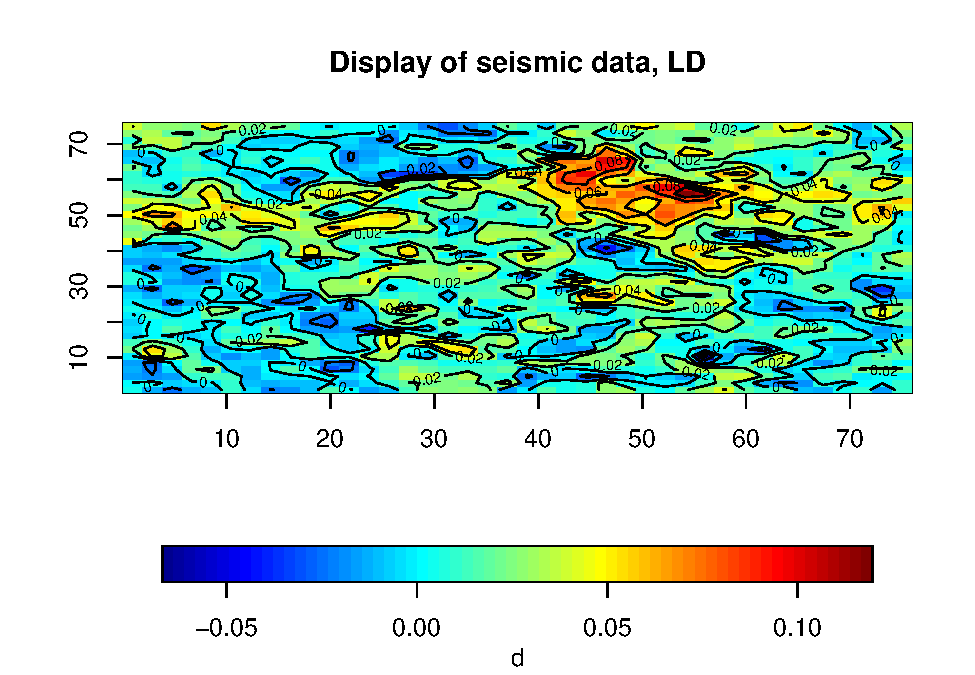
\includegraphics{Ex3_files/figure-latex/unnamed-chunk-3-1.pdf}

\begin{Shaded}
\begin{Highlighting}[]
\KeywordTok{par}\NormalTok{(}\DataTypeTok{mfrow=}\KeywordTok{c}\NormalTok{(}\DecValTok{1}\NormalTok{,}\DecValTok{1}\NormalTok{))}
\end{Highlighting}
\end{Shaded}

\begin{Shaded}
\begin{Highlighting}[]
\CommentTok{#1b}
\CommentTok{# Calculating pi-s from data. }
\NormalTok{pi <-}\StringTok{ }\KeywordTok{dnorm}\NormalTok{(seismic}\OperatorTok{$}\NormalTok{d, }\DataTypeTok{mean =} \FloatTok{0.08}\NormalTok{, }\DataTypeTok{sd =} \FloatTok{0.06}\NormalTok{)}\OperatorTok{/}\NormalTok{(}\KeywordTok{dnorm}\NormalTok{(seismic}\OperatorTok{$}\NormalTok{d, }\DataTypeTok{mean =} \FloatTok{0.02}\NormalTok{, }\DataTypeTok{sd =} \FloatTok{0.06}\NormalTok{) }\OperatorTok{+}\StringTok{ }\KeywordTok{dnorm}\NormalTok{(seismic}\OperatorTok{$}\NormalTok{d, }\DataTypeTok{mean =} \FloatTok{0.08}\NormalTok{, }\DataTypeTok{sd =} \FloatTok{0.06}\NormalTok{))}
\NormalTok{topo.li <-}\StringTok{ }\KeywordTok{interp}\NormalTok{(seismic}\OperatorTok{$}\NormalTok{x, seismic}\OperatorTok{$}\NormalTok{y, pi)}
\KeywordTok{image.plot}\NormalTok{(topo.li, }\DataTypeTok{main =} \StringTok{"Display of probabilies, LD"}\NormalTok{, }\DataTypeTok{horizontal =}\NormalTok{ T, }\DataTypeTok{legend.lab =} \StringTok{"p"}\NormalTok{)}
\KeywordTok{contour}\NormalTok{(topo.li,}\DataTypeTok{add=}\NormalTok{T)}
\end{Highlighting}
\end{Shaded}

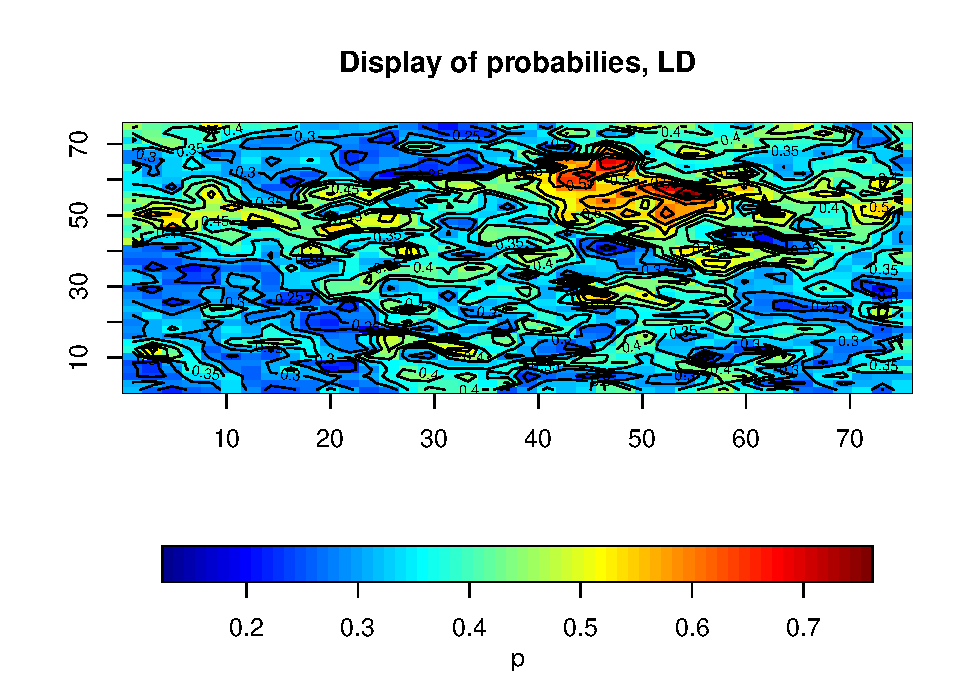
\includegraphics{Ex3_files/figure-latex/unnamed-chunk-4-1.pdf}

\begin{Shaded}
\begin{Highlighting}[]
\KeywordTok{par}\NormalTok{(}\DataTypeTok{mfrow=}\KeywordTok{c}\NormalTok{(}\DecValTok{1}\NormalTok{,}\DecValTok{1}\NormalTok{))}
\end{Highlighting}
\end{Shaded}

\begin{Shaded}
\begin{Highlighting}[]
\KeywordTok{par}\NormalTok{(}\DataTypeTok{oma =} \KeywordTok{c}\NormalTok{(}\DecValTok{4}\NormalTok{, }\DecValTok{1}\NormalTok{, }\DecValTok{1}\NormalTok{, }\DecValTok{1}\NormalTok{))}

\NormalTok{simulate.unif <-}\StringTok{ }\ControlFlowTok{function}\NormalTok{()\{}
  \KeywordTok{sapply}\NormalTok{(pi, }\ControlFlowTok{function}\NormalTok{(p) }\KeywordTok{rbinom}\NormalTok{(}\DataTypeTok{n =} \DecValTok{1}\NormalTok{, }\DataTypeTok{size =} \DecValTok{1}\NormalTok{, }\DataTypeTok{prob =}\NormalTok{ p))}
\NormalTok{\}}

\KeywordTok{par}\NormalTok{(}\DataTypeTok{mfrow=}\KeywordTok{c}\NormalTok{(}\DecValTok{3}\NormalTok{,}\DecValTok{2}\NormalTok{))}
\KeywordTok{set.seed}\NormalTok{(}\DecValTok{1}\NormalTok{)}
\ControlFlowTok{for}\NormalTok{(i }\ControlFlowTok{in} \DecValTok{1}\OperatorTok{:}\DecValTok{6}\NormalTok{)\{}
\NormalTok{  sim.res <-}\StringTok{ }\KeywordTok{simulate.unif}\NormalTok{()}
\NormalTok{  topo.li <-}\StringTok{ }\KeywordTok{interp}\NormalTok{(seismic}\OperatorTok{$}\NormalTok{x, seismic}\OperatorTok{$}\NormalTok{y, sim.res)}
  \KeywordTok{image}\NormalTok{(topo.li, }\DataTypeTok{nlevel =} \DecValTok{2}\NormalTok{, }\DataTypeTok{col =} \KeywordTok{c}\NormalTok{(}\StringTok{"#F7F396"}\NormalTok{, }\StringTok{"purple"}\NormalTok{), }\DataTypeTok{cex =} \DecValTok{10}\NormalTok{)}
  \KeywordTok{title}\NormalTok{(}\DataTypeTok{main =} \KeywordTok{paste0}\NormalTok{(}\StringTok{"Simulation "}\NormalTok{, i), }\DataTypeTok{font.main =} \DecValTok{12}\NormalTok{)}

\NormalTok{\}}
\end{Highlighting}
\end{Shaded}

\begin{verbatim}
## Warning in plot.window(...): "nlevel" is not a graphical parameter
\end{verbatim}

\begin{verbatim}
## Warning in plot.xy(xy, type, ...): "nlevel" is not a graphical parameter
\end{verbatim}

\begin{verbatim}
## Warning in axis(side = side, at = at, labels = labels, ...): "nlevel" is not a
## graphical parameter

## Warning in axis(side = side, at = at, labels = labels, ...): "nlevel" is not a
## graphical parameter
\end{verbatim}

\begin{verbatim}
## Warning in box(...): "nlevel" is not a graphical parameter
\end{verbatim}

\begin{verbatim}
## Warning in title(...): "nlevel" is not a graphical parameter
\end{verbatim}

\begin{verbatim}
## Warning in plot.window(...): "nlevel" is not a graphical parameter
\end{verbatim}

\begin{verbatim}
## Warning in plot.xy(xy, type, ...): "nlevel" is not a graphical parameter
\end{verbatim}

\begin{verbatim}
## Warning in axis(side = side, at = at, labels = labels, ...): "nlevel" is not a
## graphical parameter

## Warning in axis(side = side, at = at, labels = labels, ...): "nlevel" is not a
## graphical parameter
\end{verbatim}

\begin{verbatim}
## Warning in box(...): "nlevel" is not a graphical parameter
\end{verbatim}

\begin{verbatim}
## Warning in title(...): "nlevel" is not a graphical parameter
\end{verbatim}

\begin{verbatim}
## Warning in plot.window(...): "nlevel" is not a graphical parameter
\end{verbatim}

\begin{verbatim}
## Warning in plot.xy(xy, type, ...): "nlevel" is not a graphical parameter
\end{verbatim}

\begin{verbatim}
## Warning in axis(side = side, at = at, labels = labels, ...): "nlevel" is not a
## graphical parameter

## Warning in axis(side = side, at = at, labels = labels, ...): "nlevel" is not a
## graphical parameter
\end{verbatim}

\begin{verbatim}
## Warning in box(...): "nlevel" is not a graphical parameter
\end{verbatim}

\begin{verbatim}
## Warning in title(...): "nlevel" is not a graphical parameter
\end{verbatim}

\begin{verbatim}
## Warning in plot.window(...): "nlevel" is not a graphical parameter
\end{verbatim}

\begin{verbatim}
## Warning in plot.xy(xy, type, ...): "nlevel" is not a graphical parameter
\end{verbatim}

\begin{verbatim}
## Warning in axis(side = side, at = at, labels = labels, ...): "nlevel" is not a
## graphical parameter

## Warning in axis(side = side, at = at, labels = labels, ...): "nlevel" is not a
## graphical parameter
\end{verbatim}

\begin{verbatim}
## Warning in box(...): "nlevel" is not a graphical parameter
\end{verbatim}

\begin{verbatim}
## Warning in title(...): "nlevel" is not a graphical parameter
\end{verbatim}

\begin{verbatim}
## Warning in plot.window(...): "nlevel" is not a graphical parameter
\end{verbatim}

\begin{verbatim}
## Warning in plot.xy(xy, type, ...): "nlevel" is not a graphical parameter
\end{verbatim}

\begin{verbatim}
## Warning in axis(side = side, at = at, labels = labels, ...): "nlevel" is not a
## graphical parameter

## Warning in axis(side = side, at = at, labels = labels, ...): "nlevel" is not a
## graphical parameter
\end{verbatim}

\begin{verbatim}
## Warning in box(...): "nlevel" is not a graphical parameter
\end{verbatim}

\begin{verbatim}
## Warning in title(...): "nlevel" is not a graphical parameter
\end{verbatim}

\begin{verbatim}
## Warning in plot.window(...): "nlevel" is not a graphical parameter
\end{verbatim}

\begin{verbatim}
## Warning in plot.xy(xy, type, ...): "nlevel" is not a graphical parameter
\end{verbatim}

\begin{verbatim}
## Warning in axis(side = side, at = at, labels = labels, ...): "nlevel" is not a
## graphical parameter

## Warning in axis(side = side, at = at, labels = labels, ...): "nlevel" is not a
## graphical parameter
\end{verbatim}

\begin{verbatim}
## Warning in box(...): "nlevel" is not a graphical parameter
\end{verbatim}

\begin{verbatim}
## Warning in title(...): "nlevel" is not a graphical parameter
\end{verbatim}

\begin{Shaded}
\begin{Highlighting}[]
\KeywordTok{par}\NormalTok{(}\DataTypeTok{fig =} \KeywordTok{c}\NormalTok{(}\DecValTok{0}\NormalTok{, }\DecValTok{1}\NormalTok{, }\DecValTok{0}\NormalTok{, }\DecValTok{1}\NormalTok{), }\DataTypeTok{oma =} \KeywordTok{c}\NormalTok{(}\DecValTok{0}\NormalTok{, }\DecValTok{0}\NormalTok{, }\DecValTok{0}\NormalTok{, }\DecValTok{0}\NormalTok{), }\DataTypeTok{mar =} \KeywordTok{c}\NormalTok{(}\DecValTok{0}\NormalTok{, }\DecValTok{0}\NormalTok{, }\DecValTok{0}\NormalTok{, }\DecValTok{0}\NormalTok{), }\DataTypeTok{new =} \OtherTok{TRUE}\NormalTok{)}
\KeywordTok{plot}\NormalTok{(}\DecValTok{0}\NormalTok{, }\DecValTok{0}\NormalTok{, }\DataTypeTok{type =} \StringTok{"n"}\NormalTok{, }\DataTypeTok{bty =} \StringTok{"n"}\NormalTok{, }\DataTypeTok{xaxt =} \StringTok{"n"}\NormalTok{, }\DataTypeTok{yaxt =} \StringTok{"n"}\NormalTok{)}
\KeywordTok{legend}\NormalTok{(}\StringTok{"bottom"}\NormalTok{, }\KeywordTok{c}\NormalTok{(}\StringTok{"Sand"}\NormalTok{, }\StringTok{"Shale"}\NormalTok{), }\DataTypeTok{xpd =} \OtherTok{TRUE}\NormalTok{, }\DataTypeTok{horiz =} \OtherTok{TRUE}\NormalTok{, }\DataTypeTok{inset =} \KeywordTok{c}\NormalTok{(}\DecValTok{0}\NormalTok{, }
    \DecValTok{0}\NormalTok{), }\DataTypeTok{bty =} \StringTok{"n"}\NormalTok{, }\DataTypeTok{fill =} \KeywordTok{c}\NormalTok{(}\StringTok{"#F7F396"}\NormalTok{, }\StringTok{"purple"}\NormalTok{), }\DataTypeTok{cex =} \FloatTok{2.5}\NormalTok{)}
\end{Highlighting}
\end{Shaded}

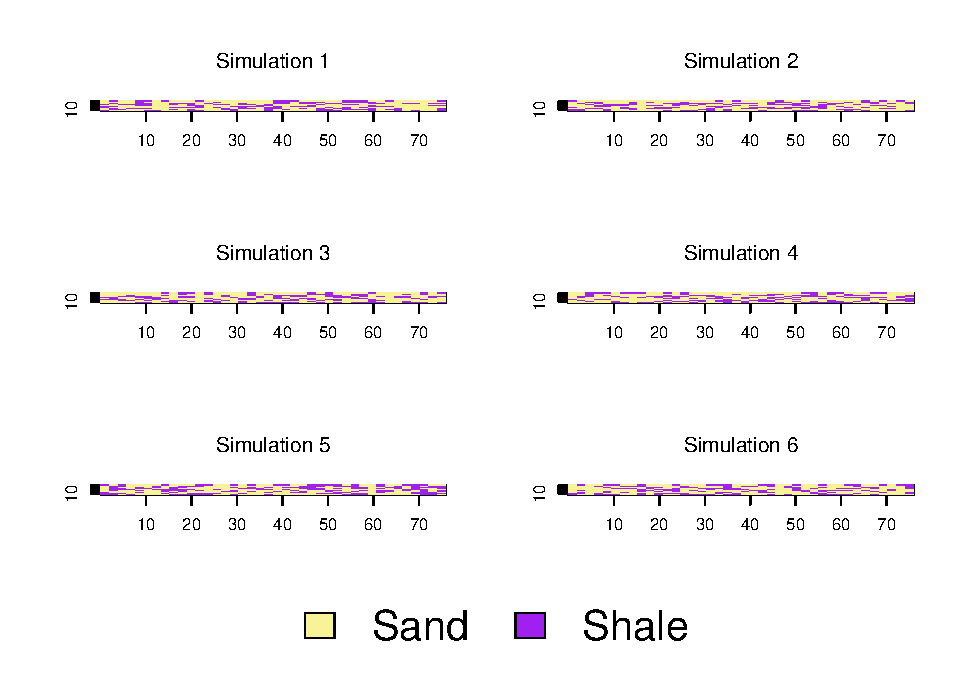
\includegraphics{Ex3_files/figure-latex/unnamed-chunk-5-1.pdf}

\begin{Shaded}
\begin{Highlighting}[]
\KeywordTok{par}\NormalTok{(}\DataTypeTok{mfrow=}\KeywordTok{c}\NormalTok{(}\DecValTok{1}\NormalTok{,}\DecValTok{1}\NormalTok{))}
\end{Highlighting}
\end{Shaded}

\begin{Shaded}
\begin{Highlighting}[]
\CommentTok{# IB MMAP expectance and variance.}
\NormalTok{ex <-}\StringTok{ }\NormalTok{pi }
\NormalTok{var <-}\StringTok{ }\NormalTok{pi}\OperatorTok{*}\NormalTok{(}\DecValTok{1}\OperatorTok{-}\NormalTok{pi)}
\NormalTok{MMAP <-}\StringTok{ }\NormalTok{pi }\OperatorTok{>=}\StringTok{ }\FloatTok{0.5}
\NormalTok{MMAP <-}\StringTok{ }\KeywordTok{as.numeric}\NormalTok{(MMAP)}

\KeywordTok{par}\NormalTok{(}\DataTypeTok{mfrow=}\KeywordTok{c}\NormalTok{(}\DecValTok{3}\NormalTok{,}\DecValTok{1}\NormalTok{))}
\NormalTok{topo.li <-}\StringTok{ }\KeywordTok{interp}\NormalTok{(seismic}\OperatorTok{$}\NormalTok{x, seismic}\OperatorTok{$}\NormalTok{y, ex)}
\KeywordTok{image.plot}\NormalTok{(topo.li, }\DataTypeTok{main =} \StringTok{"Expectance, LD"}\NormalTok{, }\DataTypeTok{horizontal =}\NormalTok{ F, }\DataTypeTok{legend.lab =} \StringTok{"Expectance"}\NormalTok{)}
\KeywordTok{contour}\NormalTok{(topo.li,}\DataTypeTok{add=}\NormalTok{T)}

\NormalTok{topo.li <-}\StringTok{ }\KeywordTok{interp}\NormalTok{(seismic}\OperatorTok{$}\NormalTok{x, seismic}\OperatorTok{$}\NormalTok{y, var)}
\KeywordTok{image.plot}\NormalTok{(topo.li, }\DataTypeTok{main =} \StringTok{"Variance, LD"}\NormalTok{, }\DataTypeTok{horizontal =}\NormalTok{ F, }\DataTypeTok{legend.lab =} \StringTok{"Variance"}\NormalTok{)}
\KeywordTok{contour}\NormalTok{(topo.li,}\DataTypeTok{add=}\NormalTok{T)}
 

\NormalTok{topo.li <-}\StringTok{ }\KeywordTok{interp}\NormalTok{(seismic}\OperatorTok{$}\NormalTok{x, seismic}\OperatorTok{$}\NormalTok{y, MMAP)}
\KeywordTok{image}\NormalTok{(topo.li, }\DataTypeTok{main =} \StringTok{"MMAP"}\NormalTok{, }\DataTypeTok{nlevel =} \DecValTok{2}\NormalTok{, }\DataTypeTok{col =} \KeywordTok{c}\NormalTok{(}\StringTok{"#F7F396"}\NormalTok{, }\StringTok{"purple"}\NormalTok{))}
\end{Highlighting}
\end{Shaded}

\begin{verbatim}
## Warning in plot.window(...): "nlevel" is not a graphical parameter
\end{verbatim}

\begin{verbatim}
## Warning in plot.xy(xy, type, ...): "nlevel" is not a graphical parameter
\end{verbatim}

\begin{verbatim}
## Warning in axis(side = side, at = at, labels = labels, ...): "nlevel" is not a
## graphical parameter

## Warning in axis(side = side, at = at, labels = labels, ...): "nlevel" is not a
## graphical parameter
\end{verbatim}

\begin{verbatim}
## Warning in box(...): "nlevel" is not a graphical parameter
\end{verbatim}

\begin{verbatim}
## Warning in title(...): "nlevel" is not a graphical parameter
\end{verbatim}

\begin{Shaded}
\begin{Highlighting}[]
\KeywordTok{legend}\NormalTok{(}\StringTok{"bottom"}\NormalTok{, }\KeywordTok{c}\NormalTok{(}\StringTok{"Sand"}\NormalTok{, }\StringTok{"Shale"}\NormalTok{), }\DataTypeTok{xpd =} \OtherTok{TRUE}\NormalTok{, }\DataTypeTok{horiz =} \OtherTok{TRUE}\NormalTok{, }\DataTypeTok{inset =} \KeywordTok{c}\NormalTok{(}\DecValTok{0}\NormalTok{, }
    \DecValTok{0}\NormalTok{), }\DataTypeTok{bty =} \StringTok{"n"}\NormalTok{, }\DataTypeTok{fill =} \KeywordTok{c}\NormalTok{(}\StringTok{"#F7F396"}\NormalTok{, }\StringTok{"purple"}\NormalTok{), }\DataTypeTok{cex =} \DecValTok{2}\NormalTok{)}
\end{Highlighting}
\end{Shaded}

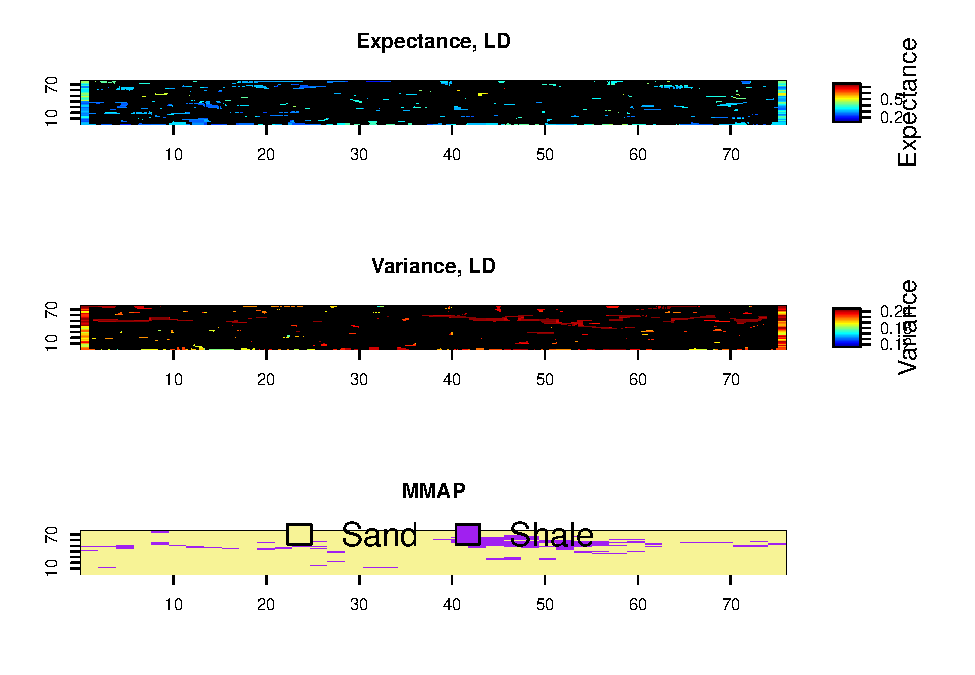
\includegraphics{Ex3_files/figure-latex/unnamed-chunk-6-1.pdf}

\begin{Shaded}
\begin{Highlighting}[]
\KeywordTok{par}\NormalTok{(}\DataTypeTok{mfrow=}\KeywordTok{c}\NormalTok{(}\DecValTok{1}\NormalTok{,}\DecValTok{1}\NormalTok{))}
\end{Highlighting}
\end{Shaded}

\begin{Shaded}
\begin{Highlighting}[]
\CommentTok{# c)}
\NormalTok{plot.map <-}\StringTok{ }\ControlFlowTok{function}\NormalTok{(df, }\DataTypeTok{title =} \StringTok{"Dc"}\NormalTok{)\{}
\NormalTok{  data <-}\StringTok{ }\KeywordTok{c}\NormalTok{()}
  \ControlFlowTok{for}\NormalTok{(i }\ControlFlowTok{in} \DecValTok{1}\OperatorTok{:}\KeywordTok{nrow}\NormalTok{(df))\{}
    \ControlFlowTok{for}\NormalTok{(j }\ControlFlowTok{in} \DecValTok{1}\OperatorTok{:}\KeywordTok{ncol}\NormalTok{(df))\{}
\NormalTok{     data <-}\StringTok{ }\KeywordTok{rbind}\NormalTok{(data, }\KeywordTok{c}\NormalTok{(i, j, df[i,j])) }
\NormalTok{    \}}
\NormalTok{  \}}
\NormalTok{  data <-}\StringTok{ }\KeywordTok{as.data.frame}\NormalTok{(data)}
  \KeywordTok{colnames}\NormalTok{(data) <-}\StringTok{ }\KeywordTok{c}\NormalTok{(}\StringTok{"x"}\NormalTok{, }\StringTok{"y"}\NormalTok{, }\StringTok{"l"}\NormalTok{)}
\NormalTok{  topo.li <-}\StringTok{ }\KeywordTok{interp}\NormalTok{(data}\OperatorTok{$}\NormalTok{x, data}\OperatorTok{$}\NormalTok{y, data}\OperatorTok{$}\NormalTok{l)}
  \KeywordTok{image}\NormalTok{(topo.li, }\DataTypeTok{main =}\NormalTok{ title, }\DataTypeTok{nlevel =} \DecValTok{2}\NormalTok{, }\DataTypeTok{col =} \KeywordTok{c}\NormalTok{(}\StringTok{"#F7F396"}\NormalTok{, }\StringTok{"purple"}\NormalTok{))}
\NormalTok{\}}
\KeywordTok{par}\NormalTok{(}\DataTypeTok{oma =} \KeywordTok{c}\NormalTok{(}\DecValTok{4}\NormalTok{, }\DecValTok{1}\NormalTok{, }\DecValTok{1}\NormalTok{, }\DecValTok{1}\NormalTok{))}
\KeywordTok{par}\NormalTok{(}\DataTypeTok{mfrow=}\KeywordTok{c}\NormalTok{(}\DecValTok{1}\NormalTok{,}\DecValTok{1}\NormalTok{))}
\KeywordTok{plot.map}\NormalTok{(complit)}
\end{Highlighting}
\end{Shaded}

\begin{verbatim}
## Warning in plot.window(...): "nlevel" is not a graphical parameter
\end{verbatim}

\begin{verbatim}
## Warning in plot.xy(xy, type, ...): "nlevel" is not a graphical parameter
\end{verbatim}

\begin{verbatim}
## Warning in axis(side = side, at = at, labels = labels, ...): "nlevel" is not a
## graphical parameter

## Warning in axis(side = side, at = at, labels = labels, ...): "nlevel" is not a
## graphical parameter
\end{verbatim}

\begin{verbatim}
## Warning in box(...): "nlevel" is not a graphical parameter
\end{verbatim}

\begin{verbatim}
## Warning in title(...): "nlevel" is not a graphical parameter
\end{verbatim}

\begin{Shaded}
\begin{Highlighting}[]
\KeywordTok{par}\NormalTok{(}\DataTypeTok{fig =} \KeywordTok{c}\NormalTok{(}\DecValTok{0}\NormalTok{, }\DecValTok{1}\NormalTok{, }\DecValTok{0}\NormalTok{, }\DecValTok{1}\NormalTok{), }\DataTypeTok{oma =} \KeywordTok{c}\NormalTok{(}\DecValTok{0}\NormalTok{, }\DecValTok{0}\NormalTok{, }\DecValTok{0}\NormalTok{, }\DecValTok{0}\NormalTok{), }\DataTypeTok{mar =} \KeywordTok{c}\NormalTok{(}\DecValTok{0}\NormalTok{, }\DecValTok{0}\NormalTok{, }\DecValTok{0}\NormalTok{, }\DecValTok{0}\NormalTok{), }\DataTypeTok{new =} \OtherTok{TRUE}\NormalTok{)}
\KeywordTok{plot}\NormalTok{(}\DecValTok{0}\NormalTok{, }\DecValTok{0}\NormalTok{, }\DataTypeTok{type =} \StringTok{"n"}\NormalTok{, }\DataTypeTok{bty =} \StringTok{"n"}\NormalTok{, }\DataTypeTok{xaxt =} \StringTok{"n"}\NormalTok{, }\DataTypeTok{yaxt =} \StringTok{"n"}\NormalTok{)}
\KeywordTok{legend}\NormalTok{(}\StringTok{"bottom"}\NormalTok{, }\KeywordTok{c}\NormalTok{(}\StringTok{"Sand"}\NormalTok{, }\StringTok{"Shale"}\NormalTok{), }\DataTypeTok{xpd =} \OtherTok{TRUE}\NormalTok{, }\DataTypeTok{horiz =} \OtherTok{TRUE}\NormalTok{, }\DataTypeTok{inset =} \KeywordTok{c}\NormalTok{(}\DecValTok{0}\NormalTok{, }
    \DecValTok{0}\NormalTok{), }\DataTypeTok{bty =} \StringTok{"n"}\NormalTok{, }\DataTypeTok{fill =} \KeywordTok{c}\NormalTok{(}\StringTok{"#F7F396"}\NormalTok{, }\StringTok{"purple"}\NormalTok{), }\DataTypeTok{cex =} \DecValTok{2}\NormalTok{)}
\end{Highlighting}
\end{Shaded}

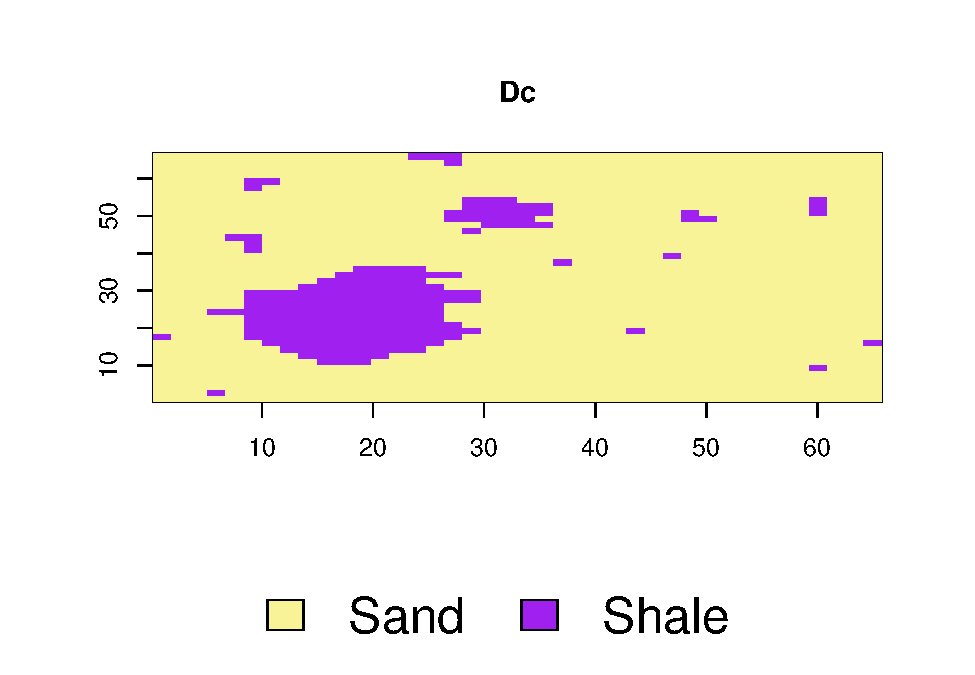
\includegraphics{Ex3_files/figure-latex/unnamed-chunk-7-1.pdf}

\begin{Shaded}
\begin{Highlighting}[]
\CommentTok{# Pseudo likelihood }
\NormalTok{mmpl <-}\StringTok{ }\ControlFlowTok{function}\NormalTok{(d, beta)\{}
\NormalTok{  res <-}\StringTok{ }\DecValTok{0}
  \ControlFlowTok{for}\NormalTok{(i }\ControlFlowTok{in} \DecValTok{1}\OperatorTok{:}\KeywordTok{nrow}\NormalTok{(d))\{}
    \ControlFlowTok{for}\NormalTok{(j }\ControlFlowTok{in} \DecValTok{1}\OperatorTok{:}\KeywordTok{ncol}\NormalTok{(d))\{}
\NormalTok{      li <-}\StringTok{ }\NormalTok{d[i, j]}
\NormalTok{      ns <-}\StringTok{ }\KeywordTok{c}\NormalTok{()}
      \ControlFlowTok{if}\NormalTok{(i }\OperatorTok{!=}\StringTok{ }\DecValTok{0}\NormalTok{)\{}
\NormalTok{        ns <-}\StringTok{ }\KeywordTok{c}\NormalTok{(ns, d[i}\DecValTok{-1}\NormalTok{,j])}
\NormalTok{      \}}
      
      \ControlFlowTok{if}\NormalTok{(i }\OperatorTok{!=}\StringTok{ }\KeywordTok{nrow}\NormalTok{(d))\{}
\NormalTok{        ns <-}\StringTok{ }\KeywordTok{c}\NormalTok{(ns, d[i}\OperatorTok{+}\DecValTok{1}\NormalTok{,j])}
\NormalTok{      \}}
      
      
      \ControlFlowTok{if}\NormalTok{(j }\OperatorTok{!=}\StringTok{ }\DecValTok{0}\NormalTok{)\{}
\NormalTok{        ns <-}\StringTok{ }\KeywordTok{c}\NormalTok{(ns, d[i,j}\DecValTok{-1}\NormalTok{])}
\NormalTok{      \}}
      
      \ControlFlowTok{if}\NormalTok{(j }\OperatorTok{!=}\StringTok{ }\KeywordTok{ncol}\NormalTok{(d))\{}
\NormalTok{        ns <-}\StringTok{ }\KeywordTok{c}\NormalTok{(ns, d[i,j}\OperatorTok{+}\DecValTok{1}\NormalTok{])}
\NormalTok{      \}}
      
\NormalTok{      ns <-}\StringTok{ }\KeywordTok{unlist}\NormalTok{(ns)}
\NormalTok{      lj.eq.to.li <-}\StringTok{ }\KeywordTok{sapply}\NormalTok{(ns, }\ControlFlowTok{function}\NormalTok{(lj) li }\OperatorTok{==}\StringTok{ }\NormalTok{lj)}
\NormalTok{      lj.eq.to}\FloatTok{.0}\NormalTok{ <-}\StringTok{ }\KeywordTok{sapply}\NormalTok{(ns, }\ControlFlowTok{function}\NormalTok{(lj) }\DecValTok{0} \OperatorTok{==}\StringTok{ }\NormalTok{lj)}
\NormalTok{      lj.eq.to}\FloatTok{.1}\NormalTok{ <-}\StringTok{ }\KeywordTok{sapply}\NormalTok{(ns, }\ControlFlowTok{function}\NormalTok{(lj) }\DecValTok{1} \OperatorTok{==}\StringTok{ }\NormalTok{lj)}
      
\NormalTok{      res <-}\StringTok{ }\NormalTok{res }\OperatorTok{+}\StringTok{ }\KeywordTok{sum}\NormalTok{(lj.eq.to.li)}\OperatorTok{*}\KeywordTok{log}\NormalTok{(beta) }\OperatorTok{-}\StringTok{ }\KeywordTok{log}\NormalTok{(beta}\OperatorTok{^}\NormalTok{(}\KeywordTok{sum}\NormalTok{(lj.eq.to}\FloatTok{.0}\NormalTok{))}\OperatorTok{+}\NormalTok{beta}\OperatorTok{^}\NormalTok{(}\KeywordTok{sum}\NormalTok{(lj.eq.to}\FloatTok{.1}\NormalTok{)))}
\NormalTok{    \}}
\NormalTok{  \}}
\NormalTok{  res}
\NormalTok{\}}

\NormalTok{mmpl.vec <-}\StringTok{ }\ControlFlowTok{function}\NormalTok{(d, bs)\{}
  \KeywordTok{sapply}\NormalTok{(bs, }\ControlFlowTok{function}\NormalTok{(b) }\KeywordTok{mmpl}\NormalTok{(}\DataTypeTok{d =}\NormalTok{ d, }\DataTypeTok{beta =}\NormalTok{ b))}
\NormalTok{\}}

\CommentTok{# Finding best estiamte using optim}
\NormalTok{opt.res <-}\StringTok{ }\KeywordTok{optim}\NormalTok{(}\DataTypeTok{fn =} \ControlFlowTok{function}\NormalTok{(bs) }\KeywordTok{mmpl.vec}\NormalTok{(complit, bs),}
      \DataTypeTok{par =} \KeywordTok{c}\NormalTok{(}\DecValTok{3}\NormalTok{),}
      \DataTypeTok{lower =} \KeywordTok{c}\NormalTok{(}\DecValTok{1}\NormalTok{),}
      \DataTypeTok{upper =} \KeywordTok{c}\NormalTok{(}\OtherTok{Inf}\NormalTok{),}
      \DataTypeTok{control=}\KeywordTok{list}\NormalTok{(}\DataTypeTok{fnscale=}\OperatorTok{-}\DecValTok{1}\NormalTok{),}
      \DataTypeTok{method =} \StringTok{"L-BFGS-B"}\NormalTok{)}
\end{Highlighting}
\end{Shaded}

\begin{Shaded}
\begin{Highlighting}[]
\CommentTok{# Set start beta parameter}
\NormalTok{beta <-}\StringTok{ }\NormalTok{opt.res}\OperatorTok{$}\NormalTok{par}
\CommentTok{# Calcukate probability of li being 1}
\NormalTok{pl.li.}\FloatTok{1.}\NormalTok{given.ns <-}\StringTok{ }\ControlFlowTok{function}\NormalTok{(ns, di) \{}
\NormalTok{  lj.eq.to}\FloatTok{.0}\NormalTok{ <-}\StringTok{ }\KeywordTok{sapply}\NormalTok{(ns, }\ControlFlowTok{function}\NormalTok{(lj) }\DecValTok{0} \OperatorTok{==}\StringTok{ }\NormalTok{lj)}
\NormalTok{  lj.eq.to}\FloatTok{.1}\NormalTok{ <-}\StringTok{ }\KeywordTok{sapply}\NormalTok{(ns, }\ControlFlowTok{function}\NormalTok{(lj) }\DecValTok{1} \OperatorTok{==}\StringTok{ }\NormalTok{lj)}
  
  \KeywordTok{dnorm}\NormalTok{(di, }\DataTypeTok{mean =} \FloatTok{0.08}\NormalTok{, }\DataTypeTok{sd =} \FloatTok{0.06}\NormalTok{) }\OperatorTok{*}
\StringTok{    }\NormalTok{beta}\OperatorTok{^}\NormalTok{(}\KeywordTok{sum}\NormalTok{(lj.eq.to}\FloatTok{.1}\NormalTok{))}\OperatorTok{/}
\StringTok{    }\NormalTok{(beta}\OperatorTok{^}\NormalTok{(}\KeywordTok{sum}\NormalTok{(lj.eq.to}\FloatTok{.1}\NormalTok{))}\OperatorTok{*}\KeywordTok{dnorm}\NormalTok{(di, }\DataTypeTok{mean =} \FloatTok{0.08}\NormalTok{, }\DataTypeTok{sd =} \FloatTok{0.06}\NormalTok{)}\OperatorTok{+}
\StringTok{       }\NormalTok{beta}\OperatorTok{^}\NormalTok{(}\KeywordTok{sum}\NormalTok{(lj.eq.to}\FloatTok{.0}\NormalTok{))}\OperatorTok{*}\KeywordTok{dnorm}\NormalTok{(di, }\DataTypeTok{mean =} \FloatTok{0.02}\NormalTok{, }\DataTypeTok{sd =} \FloatTok{0.06}\NormalTok{))}
\NormalTok{\}}

\CommentTok{## Gibbssampler}
\CommentTok{# Sample from a cell}
\NormalTok{single.step.cell <-}\StringTok{ }\ControlFlowTok{function}\NormalTok{(i, j, l, d)\{}
\NormalTok{  di <-}\StringTok{ }\NormalTok{d[i, j]}
\NormalTok{  li <-}\StringTok{ }\NormalTok{l[i, j]}
  
  
\NormalTok{  ns <-}\StringTok{ }\KeywordTok{c}\NormalTok{()}
  \ControlFlowTok{if}\NormalTok{(i }\OperatorTok{!=}\StringTok{ }\DecValTok{0}\NormalTok{)\{}
\NormalTok{    ns <-}\StringTok{ }\KeywordTok{c}\NormalTok{(ns, l[i}\DecValTok{-1}\NormalTok{,j])}
\NormalTok{  \}}
  
  \ControlFlowTok{if}\NormalTok{(i }\OperatorTok{!=}\StringTok{ }\KeywordTok{nrow}\NormalTok{(l))\{}
\NormalTok{    ns <-}\StringTok{ }\KeywordTok{c}\NormalTok{(ns, l[i}\OperatorTok{+}\DecValTok{1}\NormalTok{,j])}
\NormalTok{  \}}
  
  
  \ControlFlowTok{if}\NormalTok{(j }\OperatorTok{!=}\StringTok{ }\DecValTok{0}\NormalTok{)\{}
\NormalTok{    ns <-}\StringTok{ }\KeywordTok{c}\NormalTok{(ns, l[i,j}\DecValTok{-1}\NormalTok{])}
\NormalTok{  \}}
  
  \ControlFlowTok{if}\NormalTok{(j }\OperatorTok{!=}\StringTok{ }\KeywordTok{ncol}\NormalTok{(l))\{}
\NormalTok{    ns <-}\StringTok{ }\KeywordTok{c}\NormalTok{(ns, l[i,j}\OperatorTok{+}\DecValTok{1}\NormalTok{])}
\NormalTok{  \}}
  
  \CommentTok{# Chance translate to 1 }
\NormalTok{  p <-}\StringTok{ }\KeywordTok{pl.li.1.given.ns}\NormalTok{(ns, di)}
\NormalTok{  li.next <-}\StringTok{ }\KeywordTok{rbinom}\NormalTok{(}\DataTypeTok{n =} \DecValTok{1}\NormalTok{, }\DataTypeTok{size =} \DecValTok{1}\NormalTok{, }\DataTypeTok{prob =}\NormalTok{ p)}
  
\NormalTok{  l[i, j] <-}\StringTok{ }\NormalTok{li.next}
  \KeywordTok{return}\NormalTok{(l)}
\NormalTok{\}}

\CommentTok{# Sweep a single time}
\NormalTok{single.step <-}\StringTok{ }\ControlFlowTok{function}\NormalTok{(l, d)\{}
  \ControlFlowTok{for}\NormalTok{(i }\ControlFlowTok{in} \DecValTok{1}\OperatorTok{:}\KeywordTok{nrow}\NormalTok{(l))\{}
    \ControlFlowTok{for}\NormalTok{(j }\ControlFlowTok{in} \DecValTok{1}\OperatorTok{:}\KeywordTok{ncol}\NormalTok{(l))\{}
\NormalTok{      i <-}\StringTok{ }\KeywordTok{sample}\NormalTok{(}\KeywordTok{nrow}\NormalTok{(l), }\DataTypeTok{size =} \DecValTok{1}\NormalTok{)}
\NormalTok{      j <-}\StringTok{ }\KeywordTok{sample}\NormalTok{(}\KeywordTok{ncol}\NormalTok{(l), }\DataTypeTok{size =} \DecValTok{1}\NormalTok{)}
\NormalTok{      l <-}\StringTok{ }\KeywordTok{single.step.cell}\NormalTok{(i, j, l, d)}
\NormalTok{    \}}
\NormalTok{  \}}
  
  \KeywordTok{return}\NormalTok{(l)}
\NormalTok{\}}

\NormalTok{d <-}\StringTok{ }\KeywordTok{matrix}\NormalTok{(}\OtherTok{NA}\NormalTok{, }\DataTypeTok{nrow =} \DecValTok{75}\NormalTok{, }\DataTypeTok{ncol =} \DecValTok{75}\NormalTok{)}

\ControlFlowTok{for}\NormalTok{(i }\ControlFlowTok{in} \DecValTok{1}\OperatorTok{:}\KeywordTok{nrow}\NormalTok{(seismic))\{}
\NormalTok{  d[seismic[i,]}\OperatorTok{$}\NormalTok{x,seismic[i,]}\OperatorTok{$}\NormalTok{y] <-}\StringTok{ }\NormalTok{seismic[i,]}\OperatorTok{$}\NormalTok{d}
\NormalTok{\}}

\NormalTok{m <-}\StringTok{ }\DecValTok{250}
\CommentTok{# Sweep m times}
\NormalTok{gibbs.sampler <-}\StringTok{ }\ControlFlowTok{function}\NormalTok{(l, m, d)\{}
\NormalTok{  ls <-}\StringTok{ }\KeywordTok{c}\NormalTok{()}
  \ControlFlowTok{for}\NormalTok{(q }\ControlFlowTok{in} \DecValTok{1}\OperatorTok{:}\NormalTok{m)\{}
    \KeywordTok{print}\NormalTok{(q)}
\NormalTok{    l <-}\StringTok{ }\KeywordTok{single.step}\NormalTok{(l, d)}
\NormalTok{    ls <-}\StringTok{ }\KeywordTok{c}\NormalTok{(ls, }\KeywordTok{sum}\NormalTok{(l))}
\NormalTok{  \}}
  \KeywordTok{list}\NormalTok{(}\DataTypeTok{l =}\NormalTok{ l, }\DataTypeTok{ls =}\NormalTok{ ls)}
\NormalTok{\}}



\CommentTok{# Run m steps with different initial values}
\CommentTok{# ALl 1}
 \CommentTok{# l <- matrix(1, nrow = 75, ncol = 75)}
 \CommentTok{# res1 <- gibbs.sampler(l, m, d)}
 \CommentTok{# }
  \CommentTok{# Store number of ls in each step, in data frame}
\CommentTok{# res <- res1$ls }
\CommentTok{# all.res <- as.data.frame(res)}
\CommentTok{# all.res$x <- 1:m}
\CommentTok{# all.res$l <- "All 1"}
\CommentTok{# # All 0}
\CommentTok{# l <- matrix(0, nrow = 75, ncol = 75)}
\CommentTok{# res0 <- gibbs.sampler(l, m, d)}
\CommentTok{# # Add number of ls in each step, in data frame}
\CommentTok{# res <- res0$ls}
\CommentTok{# temp.res <- as.data.frame(res)}
\CommentTok{# temp.res$x <- 1:m}
\CommentTok{# temp.res$l <- "All 0"}
\CommentTok{# all.res <- rbind(all.res, temp.res)}
\CommentTok{# # Random with 0.5 probabilit}
\CommentTok{# set.seed(123)}
\CommentTok{# l <- matrix(rbinom(prob = 0.5, n = 75*75, size = 1), nrow = 75, ncol = 75)}
\CommentTok{# res.rand <- gibbs.sampler(l, m, d)}
\CommentTok{# # Add number of ls in each step, in data frame}
\CommentTok{# res <- res.rand$ls}
\CommentTok{# temp.res <- as.data.frame(res)}
\CommentTok{# temp.res$x <- 1:m}
\CommentTok{# temp.res$l <- "Random matrix"}
\CommentTok{# all.res <- rbind(all.res, temp.res)}
\CommentTok{# Save results}
\CommentTok{#save(all.res, file = "gibbsinitials.RData")}
\CommentTok{# Load results, uncomment above if you like to watch paint dry }
\KeywordTok{load}\NormalTok{(}\DataTypeTok{file =} \StringTok{"gibbsinitials.RData"}\NormalTok{)}

\NormalTok{all.res}\OperatorTok{$}\NormalTok{l <-}\StringTok{ }\KeywordTok{as.factor}\NormalTok{(all.res}\OperatorTok{$}\NormalTok{l)}
\NormalTok{all.res}\OperatorTok{$}\NormalTok{res <-}\StringTok{ }\NormalTok{all.res}\OperatorTok{$}\NormalTok{res}\OperatorTok{/}\NormalTok{(}\DecValTok{75}\OperatorTok{*}\DecValTok{75}\NormalTok{)}
\KeywordTok{ggplot}\NormalTok{(all.res) }\OperatorTok{+}\StringTok{ }\KeywordTok{geom_line}\NormalTok{(}\KeywordTok{aes}\NormalTok{(}\DataTypeTok{x =}\NormalTok{ x, }\DataTypeTok{y =}\NormalTok{ res, }\DataTypeTok{color =}\NormalTok{ l), }\DataTypeTok{size =} \FloatTok{0.9}\NormalTok{) }\OperatorTok{+}\StringTok{ }\KeywordTok{theme_classic}\NormalTok{() }\OperatorTok{+}\StringTok{ }
\StringTok{  }\KeywordTok{ylab}\NormalTok{(}\StringTok{"Percentage with li = 1"}\NormalTok{) }\OperatorTok{+}\StringTok{ }
\StringTok{  }\KeywordTok{xlab}\NormalTok{(}\StringTok{"Number of steps from initial"}\NormalTok{) }\OperatorTok{+}\StringTok{ }
\StringTok{  }\KeywordTok{ggtitle}\NormalTok{(}\StringTok{"Convergnce w/ different initial, percentage li = 1"}\NormalTok{)}
\end{Highlighting}
\end{Shaded}

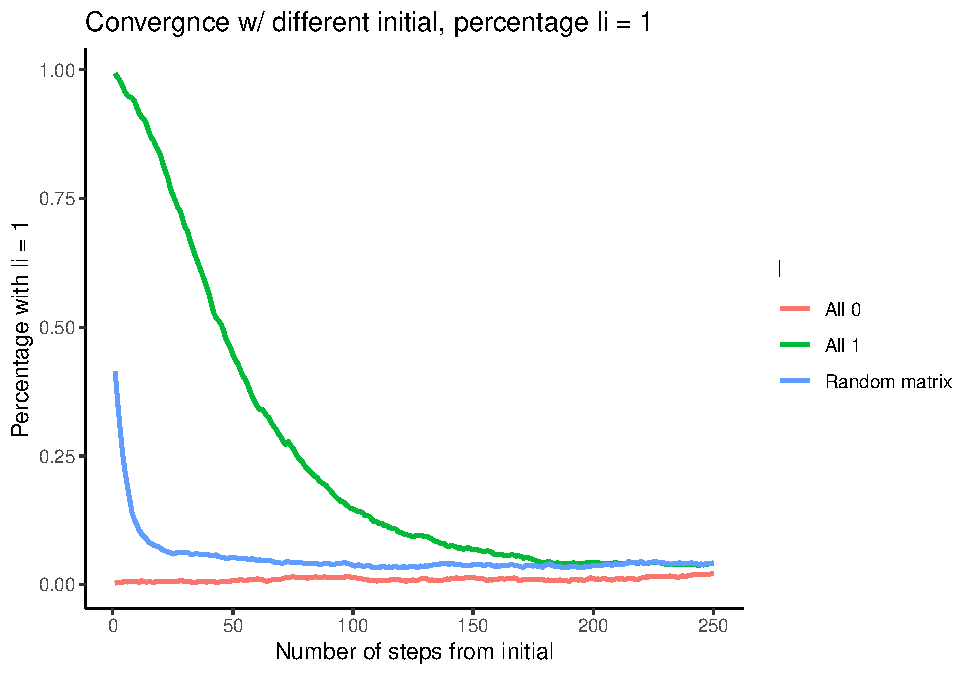
\includegraphics{Ex3_files/figure-latex/unnamed-chunk-9-1.pdf}

\begin{Shaded}
\begin{Highlighting}[]
\CommentTok{# Starting with random 50-50 seems to have converged fastes, so set burnin to 50, and generate some more samples. This time storing all results}

\CommentTok{# Sweep m times and store}
\NormalTok{m <-}\StringTok{ }\DecValTok{2500}
\NormalTok{storing.gibbs.sampler <-}\StringTok{ }\ControlFlowTok{function}\NormalTok{(l, m, d)\{}
\NormalTok{  ls <-}\StringTok{ }\KeywordTok{c}\NormalTok{()}
\NormalTok{  stored.ls <-}\StringTok{ }\KeywordTok{list}\NormalTok{()}
  \ControlFlowTok{for}\NormalTok{(q }\ControlFlowTok{in} \DecValTok{1}\OperatorTok{:}\NormalTok{m)\{}
    \KeywordTok{print}\NormalTok{(q)}
\NormalTok{    l <-}\StringTok{ }\KeywordTok{single.step}\NormalTok{(l, d)}
\NormalTok{    ls <-}\StringTok{ }\KeywordTok{c}\NormalTok{(ls, }\KeywordTok{sum}\NormalTok{(l))}
\NormalTok{    stored.ls <-}\StringTok{ }\KeywordTok{c}\NormalTok{(stored.ls, }\KeywordTok{list}\NormalTok{(l))}
\NormalTok{  \}}
  \KeywordTok{list}\NormalTok{(}\DataTypeTok{l =}\NormalTok{ l, }\DataTypeTok{ls =}\NormalTok{ ls, }\DataTypeTok{stored.ls =}\NormalTok{ stored.ls)}
\NormalTok{\}}
\KeywordTok{set.seed}\NormalTok{(}\DecValTok{123}\NormalTok{)}
\NormalTok{l <-}\StringTok{ }\KeywordTok{matrix}\NormalTok{(}\KeywordTok{rbinom}\NormalTok{(}\DataTypeTok{prob =} \FloatTok{0.5}\NormalTok{, }\DataTypeTok{n =} \DecValTok{75}\OperatorTok{*}\DecValTok{75}\NormalTok{, }\DataTypeTok{size =} \DecValTok{1}\NormalTok{), }\DataTypeTok{nrow =} \DecValTok{75}\NormalTok{, }\DataTypeTok{ncol =} \DecValTok{75}\NormalTok{)}

\CommentTok{# Only run this if you have serious amount of time}
\CommentTok{#res.rand <- storing.gibbs.sampler(l, m, d)}
\CommentTok{#save(res.rand, file = "res_rand.RData")}
\KeywordTok{load}\NormalTok{(}\StringTok{"res_rand.RData"}\NormalTok{)}
\CommentTok{# set burning}
\NormalTok{burnin <-}\StringTok{ }\DecValTok{50} 

\CommentTok{# Find distance to last}
\KeywordTok{par}\NormalTok{(}\DataTypeTok{oma =} \KeywordTok{c}\NormalTok{(}\DecValTok{4}\NormalTok{, }\DecValTok{1}\NormalTok{, }\DecValTok{1}\NormalTok{, }\DecValTok{1}\NormalTok{))}
\KeywordTok{par}\NormalTok{(}\DataTypeTok{mfrow=}\KeywordTok{c}\NormalTok{(}\DecValTok{1}\NormalTok{,}\DecValTok{2}\NormalTok{), }\DataTypeTok{mar =} \KeywordTok{c}\NormalTok{(}\DecValTok{1}\NormalTok{, }\DecValTok{1}\NormalTok{, }\DecValTok{1}\NormalTok{, }\DecValTok{1}\NormalTok{))}
\KeywordTok{plot.map}\NormalTok{(res.rand}\OperatorTok{$}\NormalTok{stored.ls[[}\DecValTok{1}\NormalTok{]], }\StringTok{"Gibbs: Initial iteration"}\NormalTok{)}
\end{Highlighting}
\end{Shaded}

\begin{verbatim}
## Warning in plot.window(...): "nlevel" is not a graphical parameter
\end{verbatim}

\begin{verbatim}
## Warning in plot.xy(xy, type, ...): "nlevel" is not a graphical parameter
\end{verbatim}

\begin{verbatim}
## Warning in axis(side = side, at = at, labels = labels, ...): "nlevel" is not a
## graphical parameter

## Warning in axis(side = side, at = at, labels = labels, ...): "nlevel" is not a
## graphical parameter
\end{verbatim}

\begin{verbatim}
## Warning in box(...): "nlevel" is not a graphical parameter
\end{verbatim}

\begin{verbatim}
## Warning in title(...): "nlevel" is not a graphical parameter
\end{verbatim}

\begin{Shaded}
\begin{Highlighting}[]
\KeywordTok{plot.map}\NormalTok{(res.rand}\OperatorTok{$}\NormalTok{stored.ls[[}\DecValTok{2500}\NormalTok{]], }\StringTok{"Gibbs: Last iteration"}\NormalTok{)}
\end{Highlighting}
\end{Shaded}

\begin{verbatim}
## Warning in plot.window(...): "nlevel" is not a graphical parameter
\end{verbatim}

\begin{verbatim}
## Warning in plot.xy(xy, type, ...): "nlevel" is not a graphical parameter
\end{verbatim}

\begin{verbatim}
## Warning in axis(side = side, at = at, labels = labels, ...): "nlevel" is not a
## graphical parameter

## Warning in axis(side = side, at = at, labels = labels, ...): "nlevel" is not a
## graphical parameter
\end{verbatim}

\begin{verbatim}
## Warning in box(...): "nlevel" is not a graphical parameter
\end{verbatim}

\begin{verbatim}
## Warning in title(...): "nlevel" is not a graphical parameter
\end{verbatim}

\begin{Shaded}
\begin{Highlighting}[]
\KeywordTok{par}\NormalTok{(}\DataTypeTok{fig =} \KeywordTok{c}\NormalTok{(}\DecValTok{0}\NormalTok{, }\DecValTok{1}\NormalTok{, }\DecValTok{0}\NormalTok{, }\DecValTok{1}\NormalTok{), }\DataTypeTok{oma =} \KeywordTok{c}\NormalTok{(}\DecValTok{0}\NormalTok{, }\DecValTok{0}\NormalTok{, }\DecValTok{0}\NormalTok{, }\DecValTok{0}\NormalTok{), }\DataTypeTok{mar =} \KeywordTok{c}\NormalTok{(}\DecValTok{0}\NormalTok{, }\DecValTok{0}\NormalTok{, }\DecValTok{0}\NormalTok{, }\DecValTok{0}\NormalTok{), }\DataTypeTok{new =} \OtherTok{TRUE}\NormalTok{)}
\KeywordTok{plot}\NormalTok{(}\DecValTok{0}\NormalTok{, }\DecValTok{0}\NormalTok{, }\DataTypeTok{type =} \StringTok{"n"}\NormalTok{, }\DataTypeTok{bty =} \StringTok{"n"}\NormalTok{, }\DataTypeTok{xaxt =} \StringTok{"n"}\NormalTok{, }\DataTypeTok{yaxt =} \StringTok{"n"}\NormalTok{)}
\KeywordTok{legend}\NormalTok{(}\StringTok{"bottom"}\NormalTok{, }\KeywordTok{c}\NormalTok{(}\StringTok{"Sand"}\NormalTok{, }\StringTok{"Shale"}\NormalTok{), }\DataTypeTok{xpd =} \OtherTok{TRUE}\NormalTok{, }\DataTypeTok{horiz =} \OtherTok{TRUE}\NormalTok{, }\DataTypeTok{inset =} \KeywordTok{c}\NormalTok{(}\DecValTok{0}\NormalTok{, }
    \DecValTok{0}\NormalTok{), }\DataTypeTok{bty =} \StringTok{"n"}\NormalTok{, }\DataTypeTok{fill =} \KeywordTok{c}\NormalTok{(}\StringTok{"#F7F396"}\NormalTok{, }\StringTok{"purple"}\NormalTok{), }\DataTypeTok{cex =} \DecValTok{2}\NormalTok{)}
\end{Highlighting}
\end{Shaded}

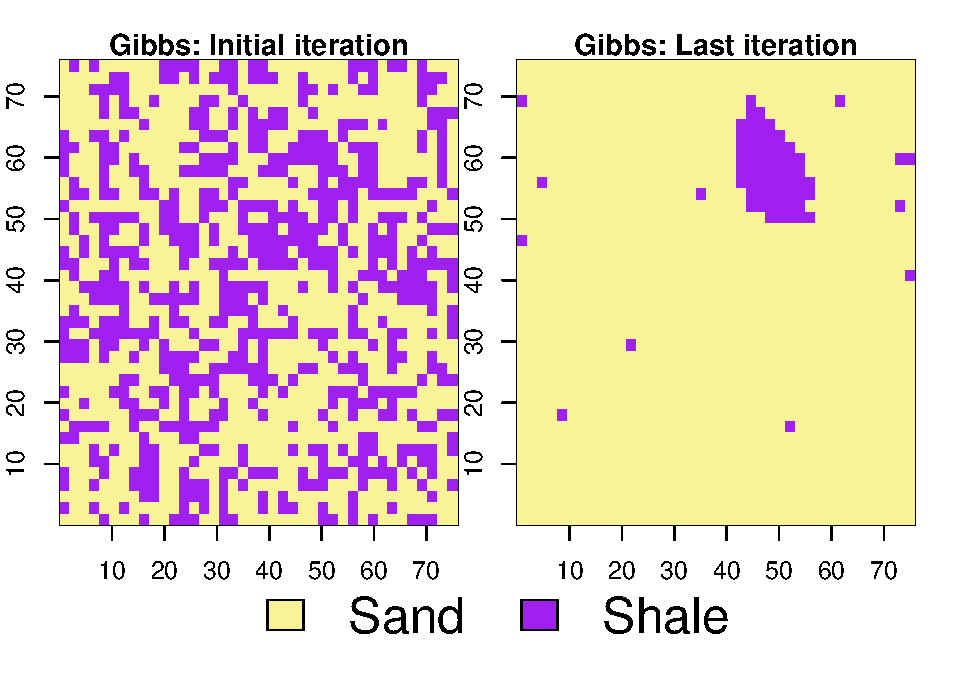
\includegraphics{Ex3_files/figure-latex/unnamed-chunk-9-2.pdf}

\begin{Shaded}
\begin{Highlighting}[]
\KeywordTok{par}\NormalTok{(opar)}
\end{Highlighting}
\end{Shaded}

\begin{verbatim}
## Warning in par(opar): graphical parameter "cin" cannot be set
\end{verbatim}

\begin{verbatim}
## Warning in par(opar): graphical parameter "cra" cannot be set
\end{verbatim}

\begin{verbatim}
## Warning in par(opar): graphical parameter "csi" cannot be set
\end{verbatim}

\begin{verbatim}
## Warning in par(opar): graphical parameter "cxy" cannot be set
\end{verbatim}

\begin{verbatim}
## Warning in par(opar): graphical parameter "din" cannot be set
\end{verbatim}

\begin{verbatim}
## Warning in par(opar): graphical parameter "page" cannot be set
\end{verbatim}

\begin{Shaded}
\begin{Highlighting}[]
\CommentTok{#Remove burnin:}
\NormalTok{res <-}\StringTok{ }\NormalTok{res.rand}\OperatorTok{$}\NormalTok{stored.ls[}\OperatorTok{-}\NormalTok{(}\DecValTok{1}\OperatorTok{:}\DecValTok{50}\NormalTok{)]}

\CommentTok{# Dont run this, it is slow}
\CommentTok{# different.df <- c()}
\CommentTok{# for(i in 1:length(res))\{}
\CommentTok{#   print(i)}
\CommentTok{#   for(j in 1:length(res))\{}
\CommentTok{#     if(i == j)\{}
\CommentTok{#       next()}
\CommentTok{#     \}}
\CommentTok{#     }
\CommentTok{#     num.different <- res[[i]] - res[[j]]}
\CommentTok{#     num.different <- abs(num.different)}
\CommentTok{#     num.different <- sum(num.different)}
\CommentTok{#     different.df <- rbind(different.df, c(num.different, abs(i-j))) }
\CommentTok{#   \}}
\CommentTok{#   }
\CommentTok{#   if(i %% 10 == 0)\{}
\CommentTok{#     write.table(different.df, "myDF.csv", sep = ",", col.names = !file.exists("myDF.csv"), append = T)}
\CommentTok{#     different.df <- c()}
\CommentTok{#   \}}
\CommentTok{#   }
\CommentTok{# \}}
\CommentTok{# }
\CommentTok{# df <- read.csv("myDF.csv")}
\CommentTok{# library(dplyr)}
\CommentTok{# head(df)}
\CommentTok{# colnames(df) <- c("index", "num.diff", "dist")}
\CommentTok{# df <- df %>% group_by(dist) %>% summarise(avg.diff = mean(num.diff)) }
\CommentTok{# save(df, file = "df.RData")}
\KeywordTok{load}\NormalTok{(}\StringTok{"df.RData"}\NormalTok{)}


\NormalTok{p1 <-}\StringTok{ }\KeywordTok{ggplot}\NormalTok{(df)}\OperatorTok{+}\StringTok{ }\KeywordTok{geom_line}\NormalTok{(}\KeywordTok{aes}\NormalTok{(}\DataTypeTok{x =}\NormalTok{ dist, }\DataTypeTok{y =}\NormalTok{ avg.diff)) }\OperatorTok{+}\StringTok{ }\KeywordTok{theme_classic}\NormalTok{() }\OperatorTok{+}\StringTok{ }\KeywordTok{xlab}\NormalTok{(}\StringTok{"Iteration differnce"}\NormalTok{) }\OperatorTok{+}\StringTok{ }\KeywordTok{ylab}\NormalTok{(}\StringTok{"Average amount of different cells in map"}\NormalTok{) }\OperatorTok{+}\StringTok{ }\KeywordTok{ggtitle}\NormalTok{(}\StringTok{"All iteration differences"}\NormalTok{)}
\NormalTok{p2 <-}\StringTok{ }\KeywordTok{ggplot}\NormalTok{(df)}\OperatorTok{+}\StringTok{ }\KeywordTok{geom_line}\NormalTok{(}\KeywordTok{aes}\NormalTok{(}\DataTypeTok{x =}\NormalTok{ dist, }\DataTypeTok{y =}\NormalTok{ avg.diff)) }\OperatorTok{+}\StringTok{ }\KeywordTok{xlim}\NormalTok{(}\KeywordTok{c}\NormalTok{(}\DecValTok{0}\NormalTok{,}\DecValTok{100}\NormalTok{)) }\OperatorTok{+}\StringTok{ }\KeywordTok{theme_classic}\NormalTok{()}\OperatorTok{+}\StringTok{ }\KeywordTok{xlab}\NormalTok{(}\StringTok{"Iteration difference"}\NormalTok{) }\OperatorTok{+}\StringTok{ }\KeywordTok{ylab}\NormalTok{(}\StringTok{"Average amount of different cells in map"}\NormalTok{) }\OperatorTok{+}\StringTok{ }\KeywordTok{ggtitle}\NormalTok{(}\StringTok{"0-100 iteration difference"}\NormalTok{)}
\NormalTok{p <-}\StringTok{ }\KeywordTok{ggarrange}\NormalTok{(p1, p2, }\DataTypeTok{ncol =} \DecValTok{2}\NormalTok{, }\DataTypeTok{nrow =} \DecValTok{1}\NormalTok{)}
\end{Highlighting}
\end{Shaded}

\begin{verbatim}
## Warning: Removed 2349 row(s) containing missing values (geom_path).
\end{verbatim}

\begin{Shaded}
\begin{Highlighting}[]
\KeywordTok{annotate_figure}\NormalTok{(p,}
                \DataTypeTok{top =} \KeywordTok{text_grob}\NormalTok{(}\StringTok{"Visualizing sample difference after n-iterations"}\NormalTok{, }\DataTypeTok{color =} \StringTok{"black"}\NormalTok{, }\DataTypeTok{face =} \StringTok{"bold"}\NormalTok{, }\DataTypeTok{size =} \DecValTok{14}\NormalTok{))}
\end{Highlighting}
\end{Shaded}

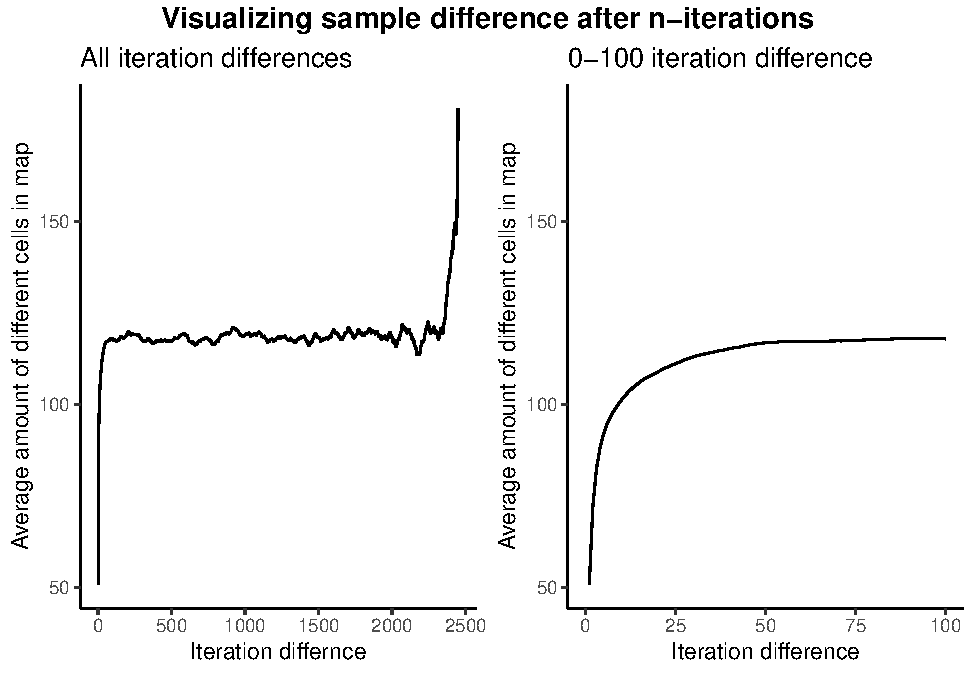
\includegraphics{Ex3_files/figure-latex/unnamed-chunk-9-3.pdf}

\begin{Shaded}
\begin{Highlighting}[]
\CommentTok{# Keep every 50th  for independence}
\NormalTok{res <-}\StringTok{ }\NormalTok{res[(}\DecValTok{1}\OperatorTok{:}\KeywordTok{length}\NormalTok{(res))[}\DecValTok{1}\OperatorTok{:}\KeywordTok{length}\NormalTok{(res) }\OperatorTok\StringTok{ }\DecValTok{50} \OperatorTok{==}\StringTok{ }\DecValTok{0}\NormalTok{]]}

\CommentTok{# number of independent samples:}
\NormalTok{m <-}\StringTok{ }\KeywordTok{length}\NormalTok{(res)}
\NormalTok{P <-}\StringTok{ }\KeywordTok{Reduce}\NormalTok{(}\StringTok{"+"}\NormalTok{, res)}
\NormalTok{P <-}\StringTok{ }\NormalTok{P}\OperatorTok{/}\NormalTok{m}
\NormalTok{P <-}\StringTok{ }\KeywordTok{as.vector}\NormalTok{(P) }\CommentTok{# row then columns}

\NormalTok{df <-}\StringTok{ }\KeywordTok{as.data.frame}\NormalTok{(P)}
\KeywordTok{names}\NormalTok{(df) <-}\StringTok{ }\KeywordTok{c}\NormalTok{(}\StringTok{"p"}\NormalTok{)}
\NormalTok{df}\OperatorTok{$}\NormalTok{x <-}\StringTok{ }\DecValTok{0}\OperatorTok{:}\NormalTok{(}\KeywordTok{nrow}\NormalTok{(seismic)}\OperatorTok{-}\DecValTok{1}\NormalTok{) }\OperatorTok\StringTok{ }\DecValTok{75} \OperatorTok{+}\StringTok{ }\DecValTok{1}
\NormalTok{df}\OperatorTok{$}\NormalTok{y <-}\StringTok{ }\DecValTok{0}\OperatorTok{:}\NormalTok{(}\KeywordTok{nrow}\NormalTok{(seismic)}\OperatorTok{-}\DecValTok{1}\NormalTok{)}\OperatorTok\StringTok{ }\DecValTok{75} \OperatorTok{+}\StringTok{ }\DecValTok{1}
\NormalTok{df}\OperatorTok{$}\NormalTok{var <-}\StringTok{ }\NormalTok{df}\OperatorTok{$}\NormalTok{p}\OperatorTok{*}\NormalTok{(}\DecValTok{1}\OperatorTok{-}\NormalTok{df}\OperatorTok{$}\NormalTok{p)}
\NormalTok{df}\OperatorTok{$}\NormalTok{mmap <-}\StringTok{ }\NormalTok{df}\OperatorTok{$}\NormalTok{p }\OperatorTok{>=}\StringTok{ }\FloatTok{0.5} 
\NormalTok{df}\OperatorTok{$}\NormalTok{mmap <-}\StringTok{ }\KeywordTok{as.numeric}\NormalTok{(df}\OperatorTok{$}\NormalTok{mmap)}

\KeywordTok{par}\NormalTok{(}\DataTypeTok{mfrow=}\KeywordTok{c}\NormalTok{(}\DecValTok{3}\NormalTok{,}\DecValTok{1}\NormalTok{), }\DataTypeTok{mar =} \KeywordTok{c}\NormalTok{(}\DecValTok{2}\NormalTok{,}\DecValTok{2}\NormalTok{,}\DecValTok{2}\NormalTok{,}\DecValTok{2}\NormalTok{))}
\NormalTok{topo.li <-}\StringTok{ }\KeywordTok{interp}\NormalTok{(df}\OperatorTok{$}\NormalTok{x, df}\OperatorTok{$}\NormalTok{y, df}\OperatorTok{$}\NormalTok{p)}
\KeywordTok{image.plot}\NormalTok{(topo.li, }\DataTypeTok{main =} \StringTok{"Expectance, LD"}\NormalTok{, }\DataTypeTok{horizontal =}\NormalTok{ F, }\DataTypeTok{legend.lab =} \StringTok{"Expectance"}\NormalTok{)}
\KeywordTok{contour}\NormalTok{(topo.li,}\DataTypeTok{add=}\NormalTok{T)}

\NormalTok{topo.li <-}\StringTok{ }\KeywordTok{interp}\NormalTok{(seismic}\OperatorTok{$}\NormalTok{x, seismic}\OperatorTok{$}\NormalTok{y, df}\OperatorTok{$}\NormalTok{var)}
\KeywordTok{image.plot}\NormalTok{(topo.li, }\DataTypeTok{main =} \StringTok{"Variance, LD"}\NormalTok{, }\DataTypeTok{horizontal =}\NormalTok{ F, }\DataTypeTok{legend.lab =} \StringTok{"Variance"}\NormalTok{)}
\KeywordTok{contour}\NormalTok{(topo.li,}\DataTypeTok{add=}\NormalTok{T)}
 

\NormalTok{topo.li <-}\StringTok{ }\KeywordTok{interp}\NormalTok{(seismic}\OperatorTok{$}\NormalTok{x, seismic}\OperatorTok{$}\NormalTok{y, df}\OperatorTok{$}\NormalTok{mmap)}
\KeywordTok{image}\NormalTok{(topo.li, }\DataTypeTok{main =} \StringTok{"MMAP"}\NormalTok{, }\DataTypeTok{nlevel =} \DecValTok{2}\NormalTok{, }\DataTypeTok{col =} \KeywordTok{c}\NormalTok{(}\StringTok{"#F7F396"}\NormalTok{, }\StringTok{"purple"}\NormalTok{))}
\end{Highlighting}
\end{Shaded}

\begin{verbatim}
## Warning in plot.window(...): "nlevel" is not a graphical parameter
\end{verbatim}

\begin{verbatim}
## Warning in plot.xy(xy, type, ...): "nlevel" is not a graphical parameter
\end{verbatim}

\begin{verbatim}
## Warning in axis(side = side, at = at, labels = labels, ...): "nlevel" is not a
## graphical parameter

## Warning in axis(side = side, at = at, labels = labels, ...): "nlevel" is not a
## graphical parameter
\end{verbatim}

\begin{verbatim}
## Warning in box(...): "nlevel" is not a graphical parameter
\end{verbatim}

\begin{verbatim}
## Warning in title(...): "nlevel" is not a graphical parameter
\end{verbatim}

\begin{Shaded}
\begin{Highlighting}[]
\KeywordTok{legend}\NormalTok{(}\StringTok{"bottom"}\NormalTok{, }\KeywordTok{c}\NormalTok{(}\StringTok{"Sand"}\NormalTok{, }\StringTok{"Shale"}\NormalTok{), }\DataTypeTok{xpd =} \OtherTok{TRUE}\NormalTok{, }\DataTypeTok{horiz =} \OtherTok{TRUE}\NormalTok{, }\DataTypeTok{inset =} \KeywordTok{c}\NormalTok{(}\DecValTok{0}\NormalTok{, }
    \DecValTok{0}\NormalTok{), }\DataTypeTok{bty =} \StringTok{"n"}\NormalTok{, }\DataTypeTok{fill =} \KeywordTok{c}\NormalTok{(}\StringTok{"#F7F396"}\NormalTok{, }\StringTok{"purple"}\NormalTok{), }\DataTypeTok{cex =} \DecValTok{2}\NormalTok{)}
\end{Highlighting}
\end{Shaded}

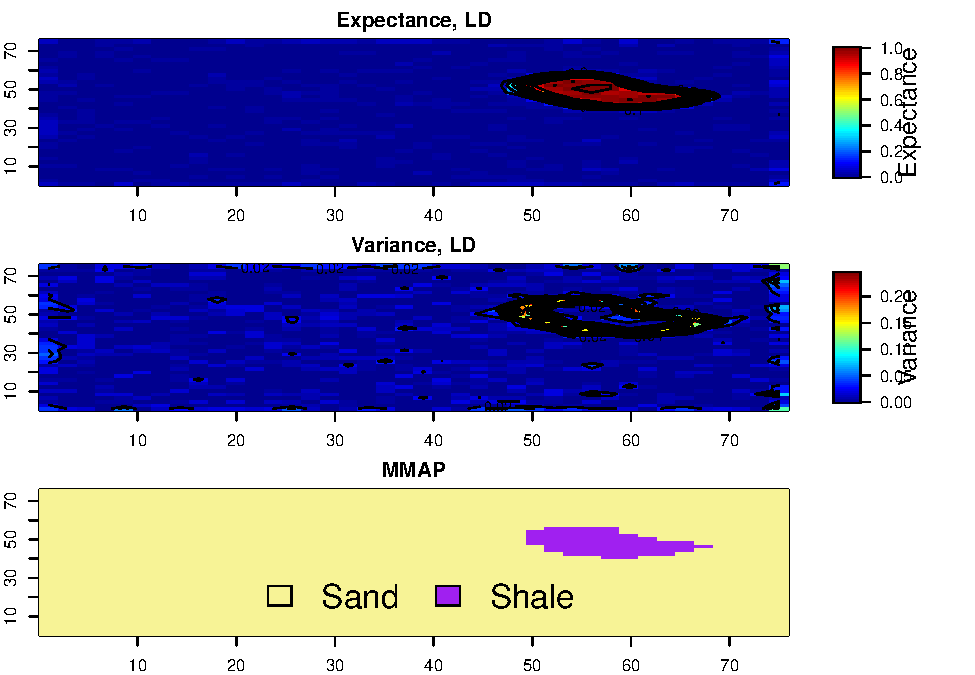
\includegraphics{Ex3_files/figure-latex/unnamed-chunk-9-4.pdf}

\begin{Shaded}
\begin{Highlighting}[]
\KeywordTok{par}\NormalTok{(}\DataTypeTok{mfrow=}\KeywordTok{c}\NormalTok{(}\DecValTok{1}\NormalTok{,}\DecValTok{1}\NormalTok{))}
\end{Highlighting}
\end{Shaded}

\end{document}
